\chapter{Introduction} 
\label{sec:Intro}
\label{chap:Intro}

Some words about why we care \cite**{Buzsaki2012,Pettersen2012,Einevoll2013,Einevoll2013a,Einevoll2019}.

%%%
\begin{figure}[!ht]
\begin{center}
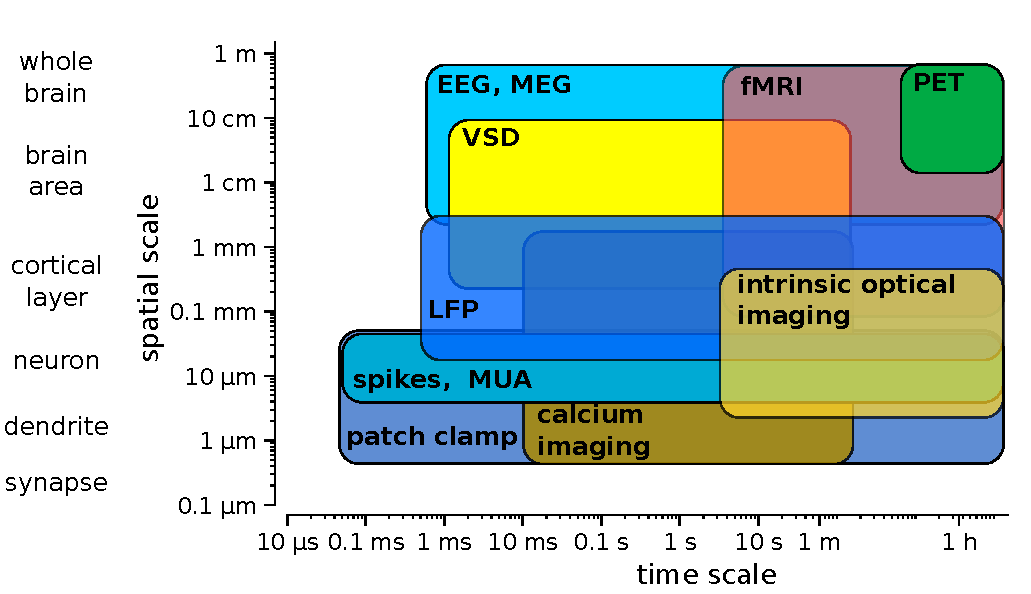
\includegraphics[width=1.0\textwidth]{Figures/Intro/measurement_scales_in_neuroscience.pdf}
\end{center}
\caption[]{\textbf{Overview of measurements of neural activity}}
\label{Intro:fig:Measurements}
\end{figure}
%%%

%%%
\begin{figure}[!ht]
\begin{center}
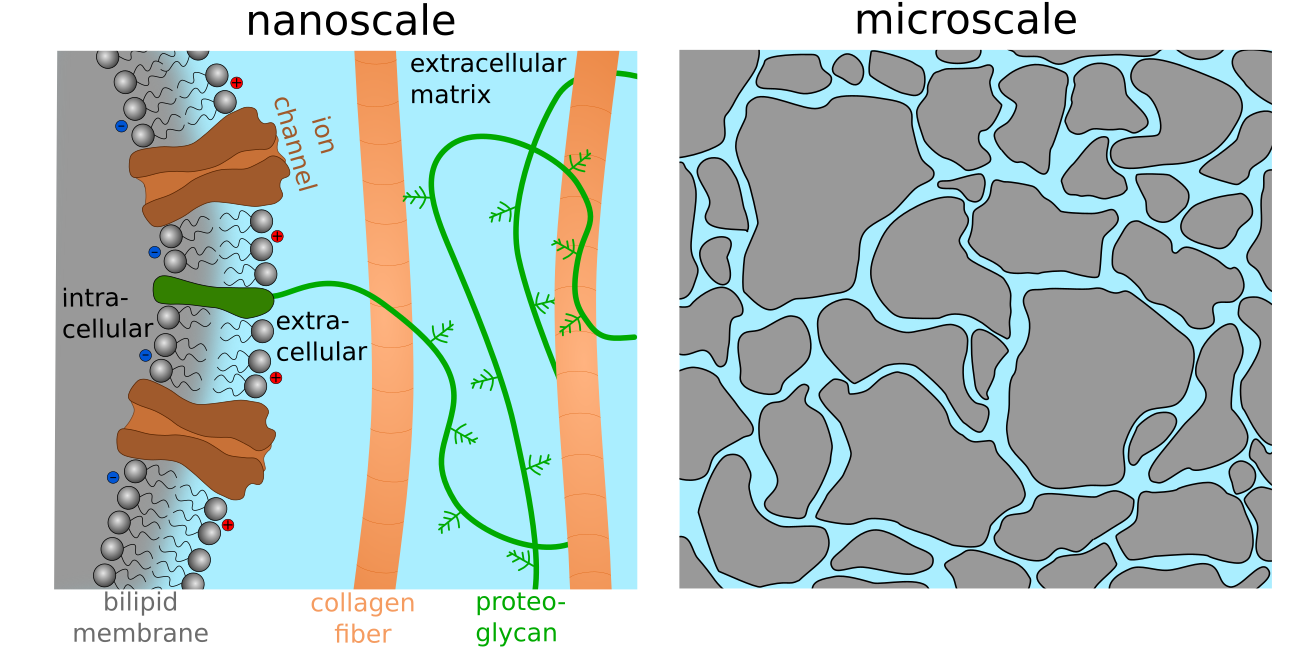
\includegraphics[width=1.0\textwidth]{Figures/Intro/ecs_nano_2.png}
\end{center}
\caption[]{\textbf{ECS}}
\label{Intro:fig:ECS-sketch}
\end{figure}
%%%

\section{\red{GH: The brain is electric}}
The main functional unit in the brain is the neuron. There are many different kinds of neurons. Some tend to increase the activity of other neurons, and these are called excitatory neurons, while others tend to decrease the activity of other neurons, and are called inhibitory neurons. Different kinds of neurons also vary in terms of their morphology. So-called pyramidal cells, for example, tend to form long nerve fibre branches (dendrites) in a preferred spatial direction, from the bottom towards the top of laminar parts of the brain, such as cortex and hippocampus. Other neurons, such as spiny stellate cells, have more spherically symmetric morphologies. The different kinds of neurons also vary in terms of their dynamical properties, i.e., in terms of how they respond to particular kinds of inputs.

As indicated in Fig. \ref{Basics:fig:Basics}A, the neural morphology can be divided into three functionally different parts: The \textit{soma}, the \textit{dendrites} and the \textit{axon}. The synapses, through which a neuron receives input from other neurons, are predominantly distributed over its dendrites, which are long and branchy extrusions from the soma. A single neuron may have synaptic connections from thousands of other neurons, and can receive input from several of them at the same time. These inputs are sensed, or "integrated" by the soma, which, depending on the net input, decides whether or not the neuron produces an output signal. The axon is another type of extrusion from the soma, which forms synapses onto the dendrites of other neurons. When the neuron produces an output signal, an electric pulse will travel along the axon and reach the synaptic location, where the (presynaptic) output from one neuron becomes the (postsynaptic) input to another. 

When a neuron rests, i.e., when it receives no input from any other neuron, its membrane potential has a negative value. The exact value varies between different neuron species, but a typical value could be $-70$ mV. When it receives inputs from other neurons, the membrane potential is jolted away from the resting potential. If the input is sufficiently strong to drive it above a certain threshold, which is often around $-50$ mV, although also this may vary between different neuron species, a set of intrinsic membrane mechanisms called ion channels will be activated. The are basically pores that open in the membrane, allowing charged particles (ions) to rush into and out from the neuron in a systematic manner to charge up and de-charge the membrane. 
The sum of these transmembrane fluxes produce a so-called action potential, a sharp spike in the voltage which peaks at some positive value of for example $+20$ mV. The action potential is the main output signal of a neuron, and the basic signaling unit in the brain.

The dynamics of the membrane potential of a neuron can be recorded experimentally with an electrode inserted into the soma of the neuron (Fig. \ref{Basics:fig:Basics}A). Such recordings will give us good insight into the dynamics of the single neuron from which it is recorded. However, if we are trying to answer some question relevant at a more systemic level, such as "how is the visual cortex processing a particular type of visual inputs?", the doings of a single neuron might not give us too much insight. 

As it is experimentally challenging to record intracellularly from more than one, or at least from more than a few, neurons at the same time, many experimental studies are instead based on using extracellular recordings. An electrode is then inserted, for example, into the brain tissue amidst the jungle of neurons that the experimentalist wants to know something about (Fig. \ref{Basics:fig:Basics}B). The signal recorded with an extracellular electrode will reflect the activity of a large number of neurons, and the interpretation of this signal is not as straightforward as the interpretation of an intracellular recording. In order to interpret extracellular recordings we therefore need a theory that relates what a population of neurons is doing to what an electrode placed amidst them, or at some distance away from them, measures. The objective of this book is present such a theory.





\section{\orange{GH: Overview the contents in this book}}
This book is divided into two parts. In Part 1 we introduce the theory for modeling neurons and the extracellular potential that they give rise to, and in Part 2 we apply this theory to extract key insights about how to interpret extracellular potentials in terms of what aspects of neural activity that they reflect.

Throughout most parts of this book, we shall compute extracellular potentials using a two-step procedure:  

\begin{itemize}
\item {\bf Step 1:} Compute the electrical activity of the cells believed to contribute to the extracellular potential. 
\item {\bf Step 2:} Compute the extracellular potential that arises from a given, underlying cellular activity.
\end{itemize}

Following this two-step procedure, Chapter \ref{sec:Neuron} describes how to model and compute the dynamics of morphologically complex neurons (step 1), and Chapter \ref{sec:VC} describes how to compute the resulting extracellular potential (step 2). The computations in step 2 depend on the extracellular medium, as reflected through its conductivity $\sigma$. Chapter \ref{sec:Sigma} is devoted to present experimental and theoretical estimates of $\sigma$, and to explain how various choices for $\sigma$ can be incorporated into the theory (step 2). Taken together, chapters \ref{sec:Neuron}-\ref{sec:Sigma} contain the theory used for all simulations in the application part (Part 2) of this book, which remains the standard theory used within the field of neuroscience to simulate extracellular potentials. 

The standard theory (covered by Chapters \ref{sec:Neuron}-\ref{sec:Sigma}) assumes (1) that ion concentrations in the extracellular (and intracellular) environment do not vary with time. This is thought to be a good approximation during normal cellular activity. However, extracellular ion concentration shifts are a trademark of many pathological conditions such as epilepsy, stroke or spreading depression \cite**{Somjen2001,Frohlich2008,Zandt2015,Ayata2015}. In Chapter \ref{sec:Eldiff} we expand step 2 by outlining a theory for modeling extracellular ion concentration dynamics surrounding active neurons, and the effects that this will have on the extracellular potential. 

The standard theory also assumes (2) that the extracellular potential (computed in step 2) does not have any feedback effect on the neurodynamics (computed in step 1). The justification making such an assumption is that $\phi$ is usually so much smaller than the membrane potential such, so-called ephaptic effects can be neglected without any severe loss in accuracy. Also, assuming this, simplifies the mathematical framework, and speeds up computations substantially. 

In reality, both in the the extracellular potential and in the extracellular ion concentrations will in principle affect the neurodynamics. Although these effects may be small for most scenarios, there are also scenarios where the assumptions (1)-(2) do not hold, so that the standard two-step procedure can not be applied. We therefore end the theory part (Part 1) of this book by giving a summary of alternative available frameworks for computing extracellular potentials and ion concentrations (Chapter \ref{sec:Schemes}).

In the application part (Part 2) of this book, we use the theory from Part 1 to simulate extracellular potentials at different levels through forward modeling. By \textit{forward modeling} we here mean that start off with a system of neurons that is supposed to mimic a physiologically realistic scenario, and then use this predict the resulting extracellular potential, i.e., a signal that one can measure experimentally. The opposite approach, \textit{inverse modeling}, would be to try to predict the system of neurons or some properties from it from a (measured) extracellular potential. \textit{Inverse modeling} is more problematic than forward modeling, as it has no unique solution, and we will not deal with this in this book.

The motivation behind forward models is multifold. Firstly, if the model system generates an extracellular potential similar to that measured in given experimental condition, it gives validity to the model system. Secondly, by manipulating aspects of the model system, such as neuronal morphology, synapse distributions, neural membrane mechanisms etc., and exploring the effects that this has on the extracellular potential, we may gain knowledge into how various aspects of neuronal dynamics are involved in shaping the extracellular potential. As such, forward modeling gives us insights that can be used to interpret experimentally recorded extracellular potentials. 

What the extracellular potential tells us about the underlying neurodynamics depends on where it was recorded, and what aspects of it that we look at, e.g., if we look at the fast variations of it (high-frequency component), or slower variations (low-frequency component). Part 2 is organized so that we first consider the extracellular potential close to its sources, i.e., amidst the forest of neurons, which can be recorded experimentally with sharp electrodes inserted into the brain tissue. By performing a filtering of this signal, we can split it into a high-frequency part and a low-frequency part. In Chapter \ref{sec:Spikes} we examine the high-frequency part, often called the multi-unit-activity (MUA), and show that this mostly reflects the population spiking activity. In In Chapter \ref{sec:LFP} we focus on the low-frequency part, and show that this mostly reflects synaptic input to populations of pyramidal cells.

In the following chapters, we study the extracellular potential at positions further away from their neuronal sources. In Chapter \ref{sec:ECoG}, we the electrocorticogram (ECoG), measured at the surface of the cortex, or the electroencephalogram (EEG) measured at the top of the scalp. We also include a chapter (Chapter \ref{sec:MEG}) on the magnetoencephalogram, which can be modeled on a framework similar to that used for EEG. 

The theory for how electrical potential propagate from neural sources to a recording electrode can, of course, also be applied to predict how signals will propagate from artificial sources such as stimulus electrodes. In Chapter \ref{sec:Stim} we briefly present a framework for this, as it will be useful in the context of understanding brain stimulations with e.g., deep electrodes. 

Finally, we discuss the state of the art technology for brain recordings, and comment on future outlooks and people like Elon Musk (Chapter \ref{sec:Tech}), before we end  by giving a summary of the main take-home messages from this book (Chapter \ref{sec:Last}).
